%%%%%%%%%%%%%%%%%%%%%%%%%%%%%%%%%%%%%%%
% a0poster Landscape Poster
% LaTeX Template
% Version 1.0 (22/06/13)
%
% The a0poster class was created by:
% Gerlinde Kettl and Matthias Weiser (tex@kettl.de)
% 
% This template has been downloaded from:
% http://www.LaTeXTemplates.com
%
% License:
% CC BY-NC-SA 3.0 (http://creativecommons.org/licenses/by-nc-sa/3.0/)
%
%%%%%%%%%%%%%%%%%%%%%%%%%%%%%%%%%%%%%%%%%

%----------------------------------------------------------------------------------------
%	PACKAGES AND OTHER DOCUMENT CONFIGURATIONS
%----------------------------------------------------------------------------------------

% maize2018 is 33'' x 46'' (84cm x 118cm)
\documentclass[maize,portrait]{a0poster}

\usepackage{fontspec}
\usepackage[svgnames]{xcolor} % enable specifying colors by their 'svgnames', for a full list of all colors available see here: http://www.latextemplates.com/svgnames-colors

% Carnegie uses Roboto Slab (serif) and Lato (sans serif)
\setmainfont[Ligatures=TeX]{Lato}

% Carnegie colors
\definecolor{CarnegiePriBlue}{cmyk}{1.00,0.85,0.15,0.25}  % main primary blue
\definecolor{CarnegieSecBlue1}{cmyk}{0.68,0.48,0.00,0.00} % first secondary blue
\definecolor{CarnegieSecBlue2}{cmyk}{0.85,0.69,0.04,0.00} % second secondary blue

\definecolor{CarnegiePriTurq}{cmyk}{0.60,0.10,0.15,0.00}  % main primary turquoise

\definecolor{CarnegiePriGreen}{cmyk}{0.46,0.00,0.90,0.00} % main primary green

\definecolor{CarnegiePriBrown}{cmyk}{0.25,0.40,0.65,0.00} % main primary brown

% multiple columns
\usepackage{multicol} % This is so we can have multiple columns of text side-by-side
\columnsep=100pt      % This is the amount of white space between the columns in the poster
\columnseprule=3pt    % This is the thickness of the black line between the columns in the poster
\def\columnseprulecolor{\color{lightgray}}

% other needed packages
\usepackage{amsfonts, amsmath, amsthm, amssymb} % For math fonts, symbols and environments
\usepackage{wrapfig}  % Allows wrapping text around tables and figures
\usepackage{graphicx} % Required for including images
\usepackage{booktabs} % Top and bottom rules for table

% tweak figure and table captions
\usepackage[font=small,labelfont={bf,color=CarnegiePriBlue},textfont={color=CarnegiePriBlue},margin=0pt,skip=18pt]{caption}

% natbib drops numbers and we'll shrink text size; drop labels
\usepackage{natbib}
\def\bibfont{\footnotesize}
\makeatletter
\renewcommand\@biblabel[1]{}
\makeatother

% tweak list spacing
\usepackage{enumitem}
\setlist[itemize]{topsep=10pt,itemsep=8pt,itemindent=48pt}
\setlist[enumerate]{topsep=10pt,itemsep=8pt,itemindent=0pt}


% tweak paragraphs
\setlength{\parindent}{0pt}
\setlength{\parskip}{12pt}

% tweak title spacing and colors
% \titlespacing{command}{left spacing}{before spacing}{after spacing}[right]
% spacing: how to read {12pt plus 4pt minus 2pt}
%          12pt is what we would like the spacing to be
%          plus 4pt means that TeX can stretch it by at most 4pt
%          minus 2pt means that TeX can shrink it by at most 2pt
\usepackage{titlesec}

% {left}{before}{after}
\titlespacing{\section}{0pt}{36pt}{12pt}
\titlespacing{\subsection}{0pt}{12pt}{12pt}
\titlespacing{\subsubsection}{0pt}{12pt}{12pt}

\titleformat{\section}{\color{CarnegiePriBlue}\Large\bfseries}{\color{CarnegiePriBlue}\thesection}{1em}{}
\titleformat{\subsection}{\color{CarnegiePriBrown}\large\bfseries}{\color{CarnegiePriBrown}\thesubsection}{1em}{}

% tweak equation whitespace
%% \abovedisplayskip=12pt plus 3pt minus 9pt
%% \abovedisplayshortskip=0pt plus 3pt
%% \belowdisplayskip=12pt plus 3pt minus 9pt
%% \belowdisplayshortskip=7pt plus 3pt minus 4pt

% width of figures for consistency
\newlength{\figwidth}
\setlength{\figwidth}{236mm}


% space above figures
\newlength{\figtopspace}
\setlength{\figtopspace}{10pt}

\graphicspath{{figures/}} % Location of the graphics files

%% % DEBUG: overlay a grid to view spacing
%\usepackage[grid,gridcolor=red!20,subgridcolor=green!20,gridunit=in]{eso-pic}

\begin{document}

%----------------------------------------------------------------------------------------
%	POSTER HEADER 
%----------------------------------------------------------------------------------------

% The header is divided into three boxes:
% The first is 55% wide and houses the title, subtitle, names and university/organization
% The second is 25% wide and houses contact information
% The third is 19% wide and houses a logo for your university/organization or a photo of you
% The widths of these boxes can be easily edited to accommodate your content as you see fit
% Note: no line breaks between minipage environments!

\textbf{\color{CarnegiePriBlue} \Huge GBS identification of genomic loci associated with polyembryony in \textit{ig1} mutants}    % Title

\begin{minipage}[m]{0.06\linewidth}
  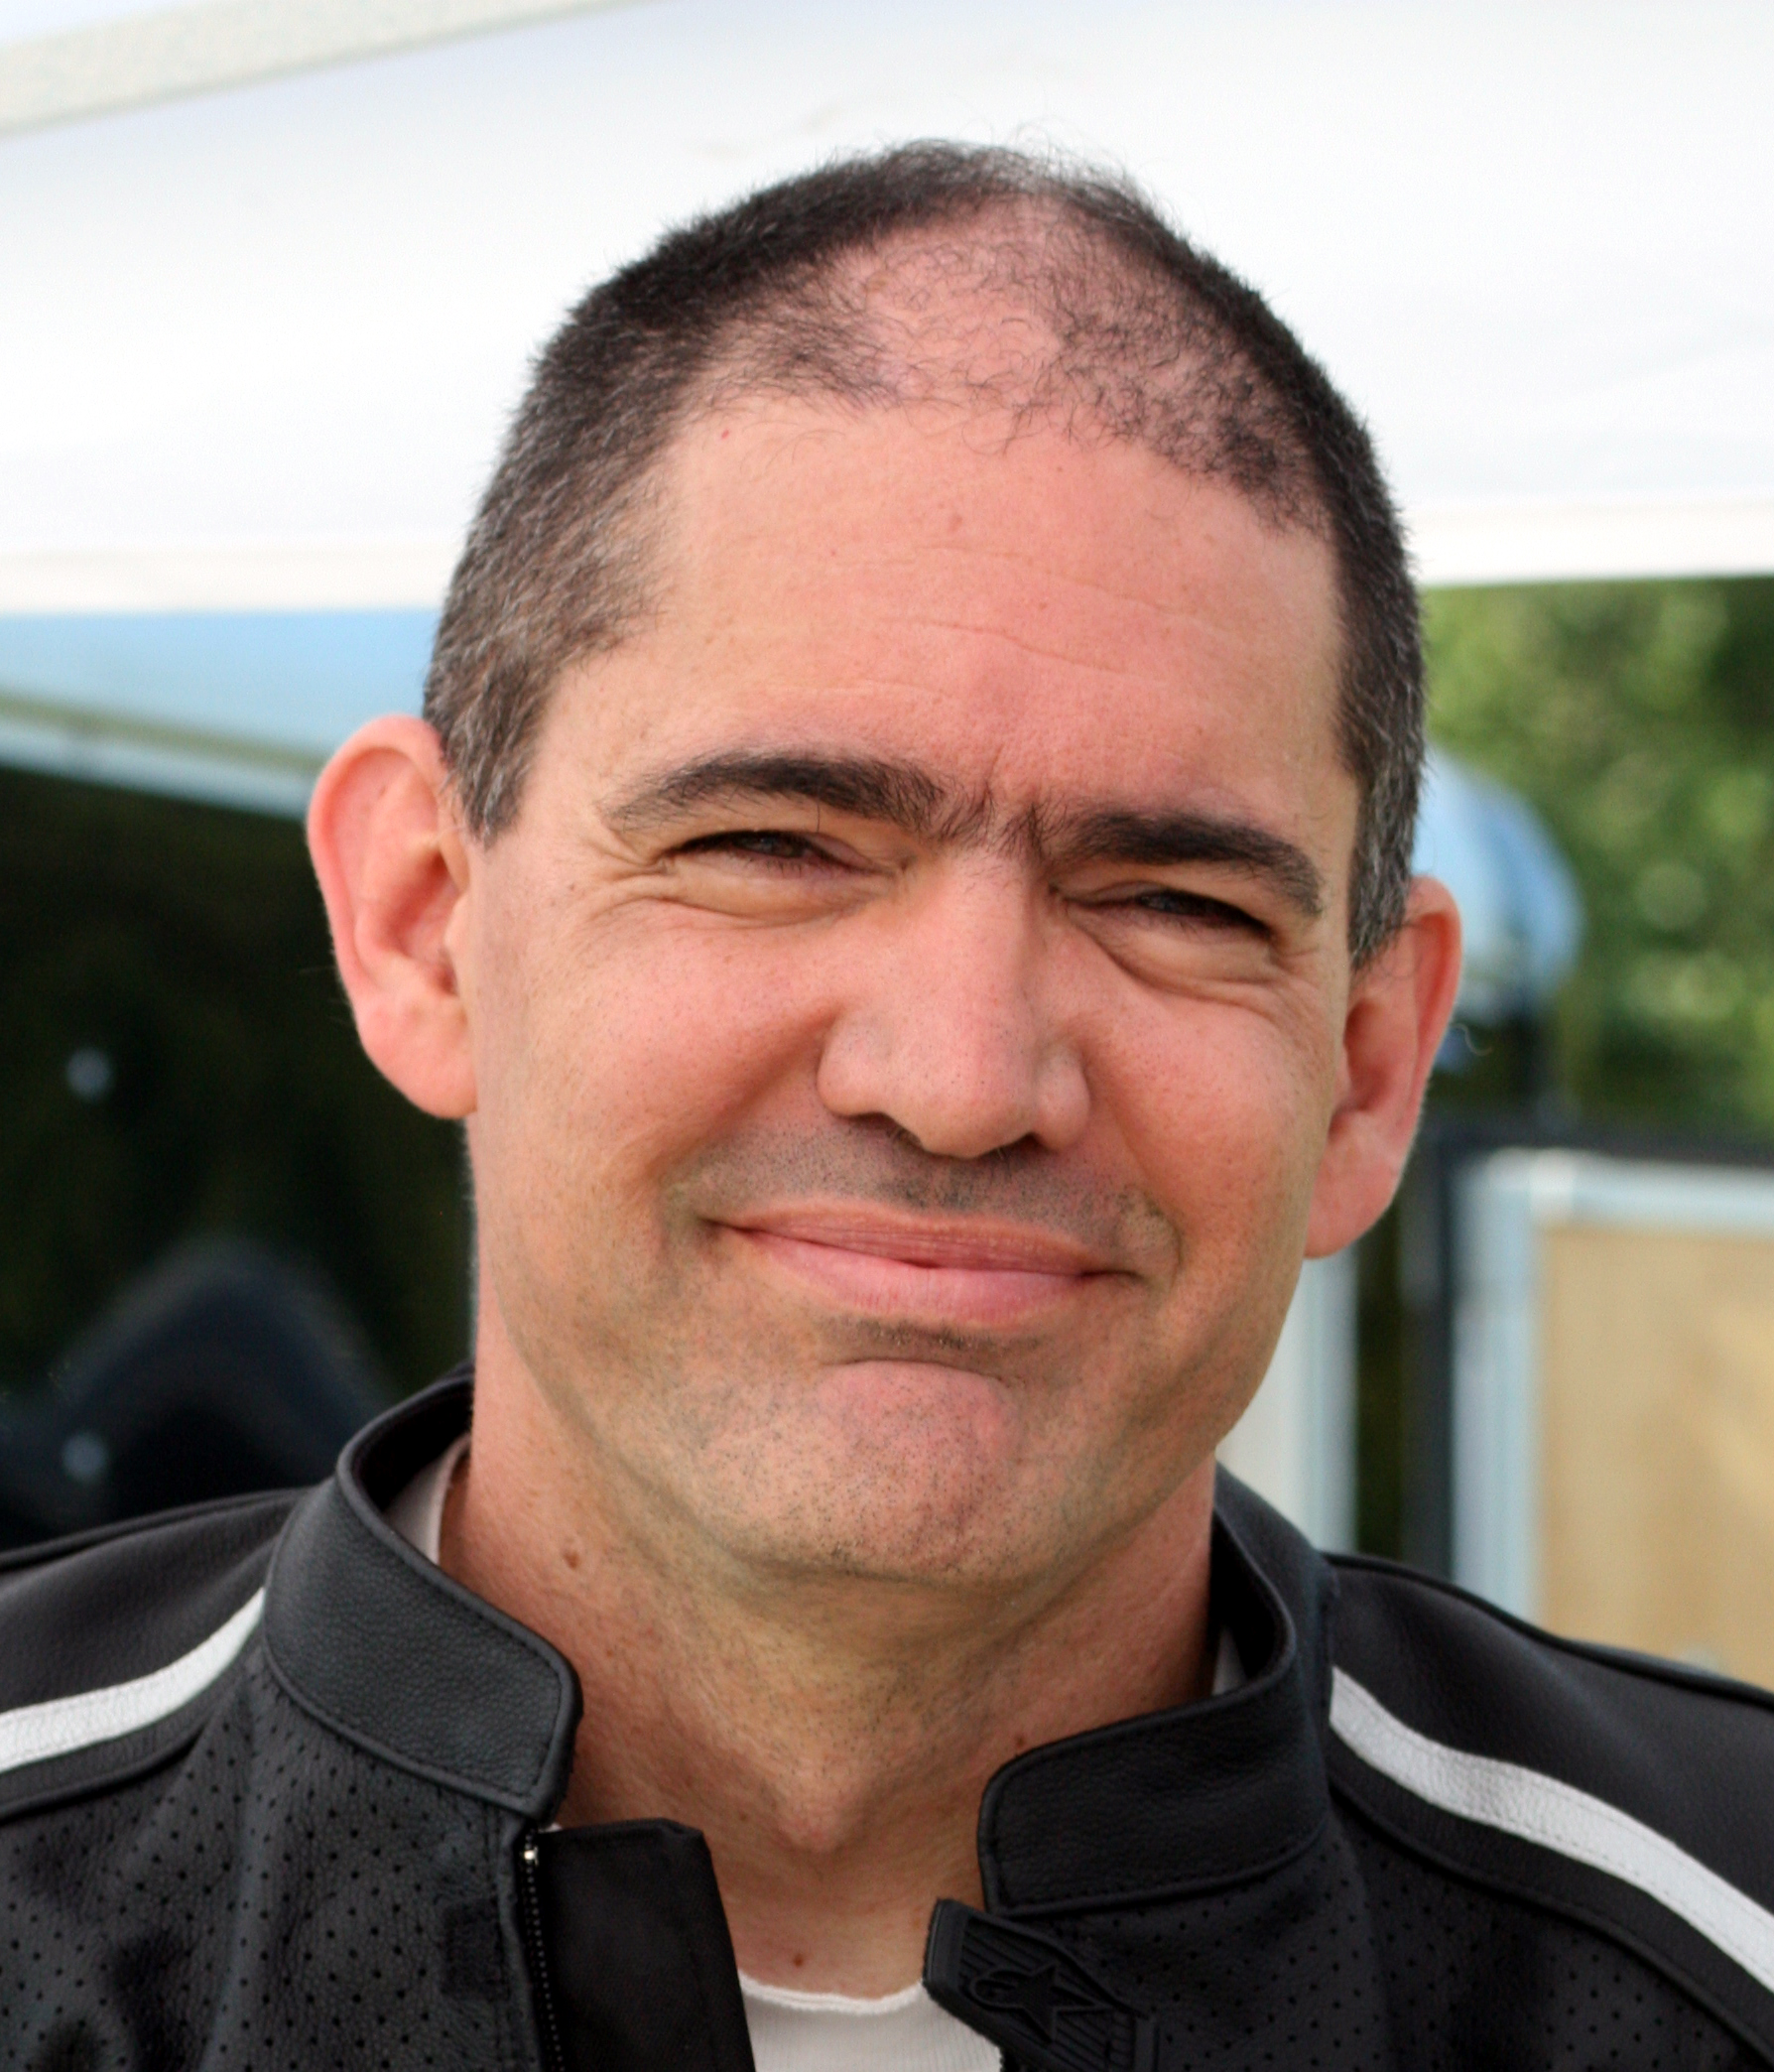
\includegraphics[height=50mm]{sam-bfr-smiling-crop.jpg} % author photo
  \hfill
\end{minipage}
\begin{minipage}[m]{0.40\linewidth}                      % Author(s)
  \color{Black}
  \Large \textbf{Sam Hokin, Matt Evans, Antony Chettoor \& Vicki Tang}
  \large shokin@carnegiescience.edu
\end{minipage}
\hfill
\begin{minipage}[m]{0.50\linewidth}                      % Author(s)
  \hfill
  
\includegraphics[height=50mm]{CS_plantbio_logo_horz.eps} % Carnegie DPB logo
\end{minipage}

\vspace{5mm} % A bit of extra whitespace between the header and poster content
\color{CarnegiePriBlue}
\hrulefill

\color{Black}

%% \color{DarkSlateGray}\Large \textbf{Contact Information:}\\
%% Department Name\\ % Address
%% University Name\\
%% 123 Broadway, State, Country\\\\
%% Phone: +1 (000) 111 1111\\ % Phone number
%% Email: \texttt{john@LaTeXTemplates.com}\\ % Email address


%----------------------------------------------------------------------------------------

\begin{multicols}{3} % This is how many columns your poster will be broken into, a poster with many figures may benefit from less columns whereas a text-heavy poster benefits from more
  \color{Black} % default color
  
  %----------------------------------------------------------------------------------------
  %	ABSTRACT
  %----------------------------------------------------------------------------------------

  %% \begin{abstract}
  %% \end{abstract}

  %----------------------------------------------------------------------------------------
  %	INTRODUCTION
  %----------------------------------------------------------------------------------------

  \section*{SUMMARY}

  The \textit{LBD6} or \textit{ASYMMETRIC LEAVES2} gene in maize is an important regulator in
  the transition from proliferation to differentiation in embryo sac development (Evans, 2007). The mutant, also
  known as \textit{indeterminate gametophyte1} (\textit{ig1}), produces
  embryo sacs which \underline{lack} the ability to \underline{limit} proliferation, leading to structural defects. These
  defects include embryo sacs with extra egg cells, extra central cells, and extra polar
  nuclei, which give rise to abnormal seed phenotypes post-fertilization. Extra egg cells in
  an embryo sac can be fertilized producing kernels with multiple viable embryos.

  The \textit{ig1-O} mutation results in different frequencies of multiple embryos, or 'twinning,' in
  different maize inbred backgrounds. Confocal microscopy confirms that Mo17 embryo
  sacs carrying the \textit{ig1-O} allele have a significantly higher frequency of multiple egg cells
  than \textit{ig1-O} embryo sacs in a B73 inbred background. The frequency of twinning is
  intermediate in the \textit{ig1-O/+} Mo17/B73 hybrid compared to \textit{ig1-O} inbred lines. This
  suggests that a genetic modifier(s) may be responsible for the difference in phenotypic
  frequency between these inbred lines.

  Genotyping By Sequencing (GBS) data analysis and initial SSR marker fine mapping indicate broad enhancers of twinning on
  chromosomes 3 and 9, as well as narrow regions elsewhere.
  
  Carrying the Mo17 allele appears to be sufficient to increase the frequency of twinning caused by the \textit{ig1-O} mutation.

  \section*{PHENOTYPES}

  The \textit{ig1} mutant produces many seeds with twin embryos (as well as triplets and other abnormalities), especially on a Mo17 background.

  \begin{center}
    \begin{minipage}[t]{1.0\linewidth}
      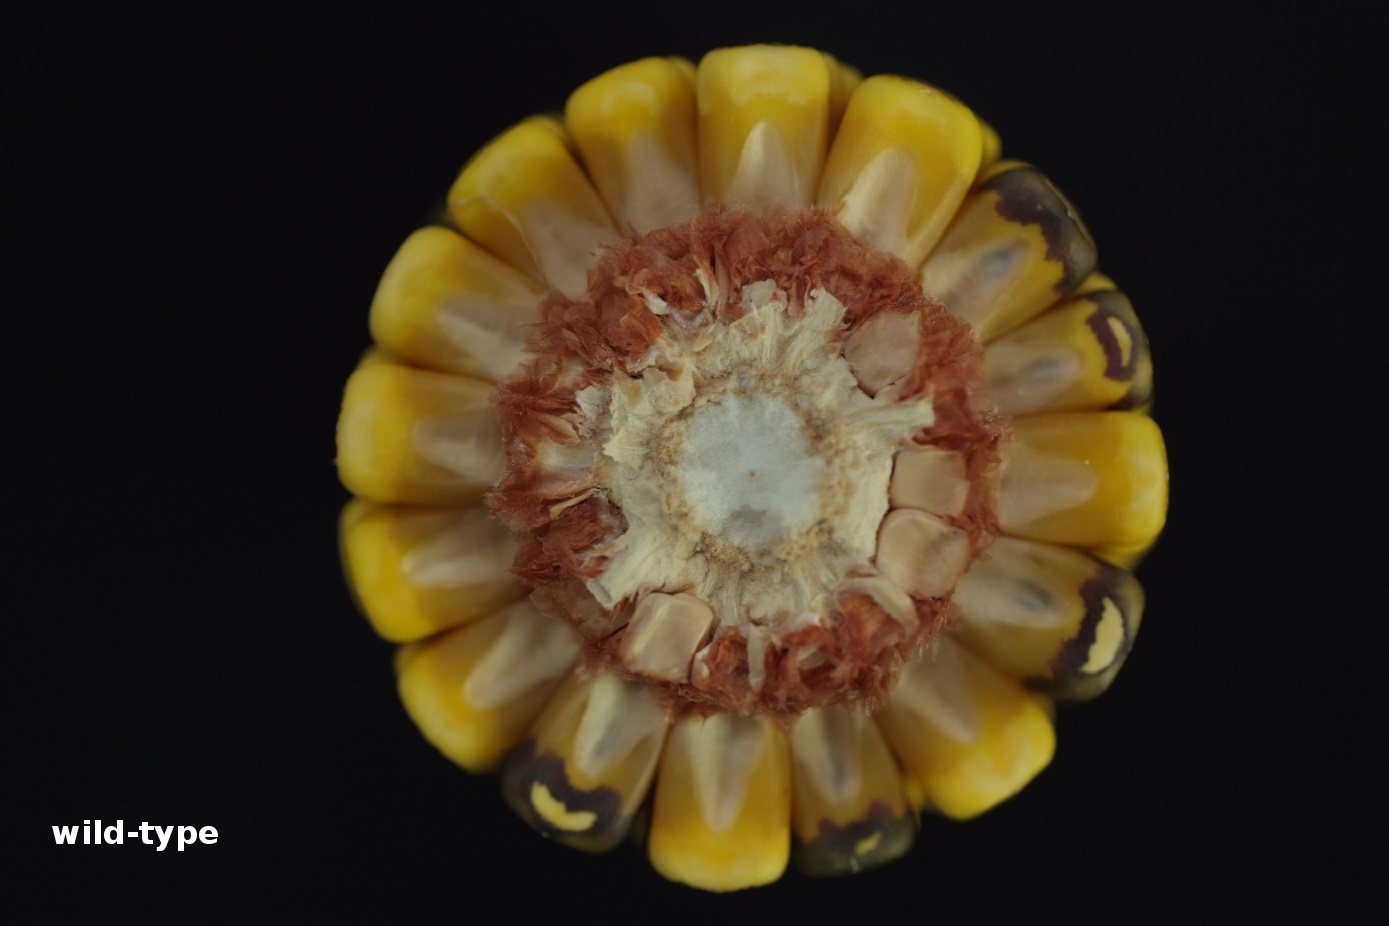
\includegraphics[width=0.5\figwidth]{Tang-ear-wt-end}
      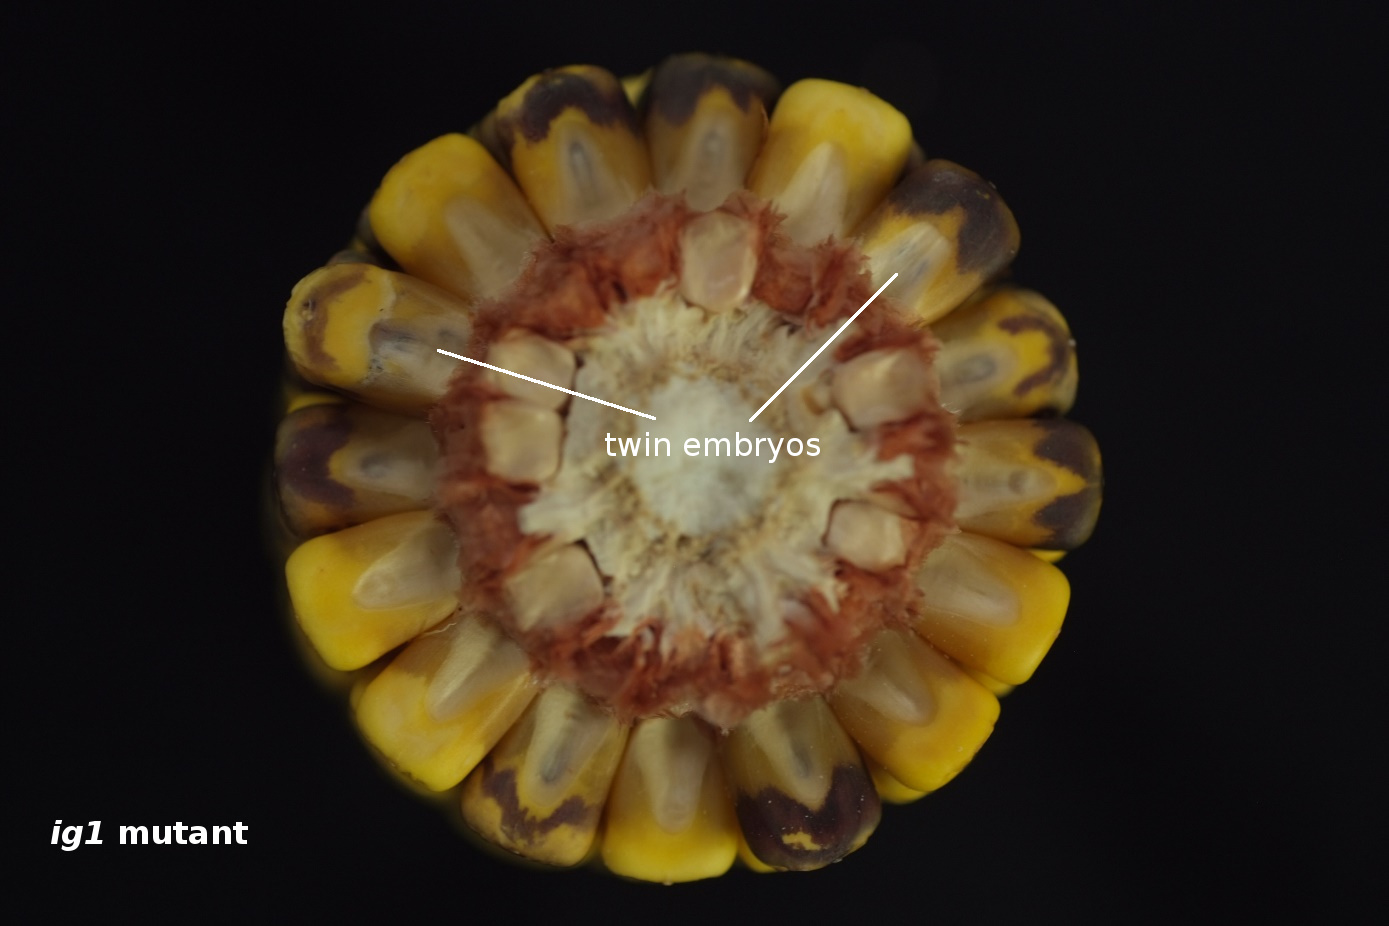
\includegraphics[width=0.5\figwidth]{Tang-ear-ig1-end}
    \end{minipage}
    \begin{minipage}[t]{1.0\linewidth}
      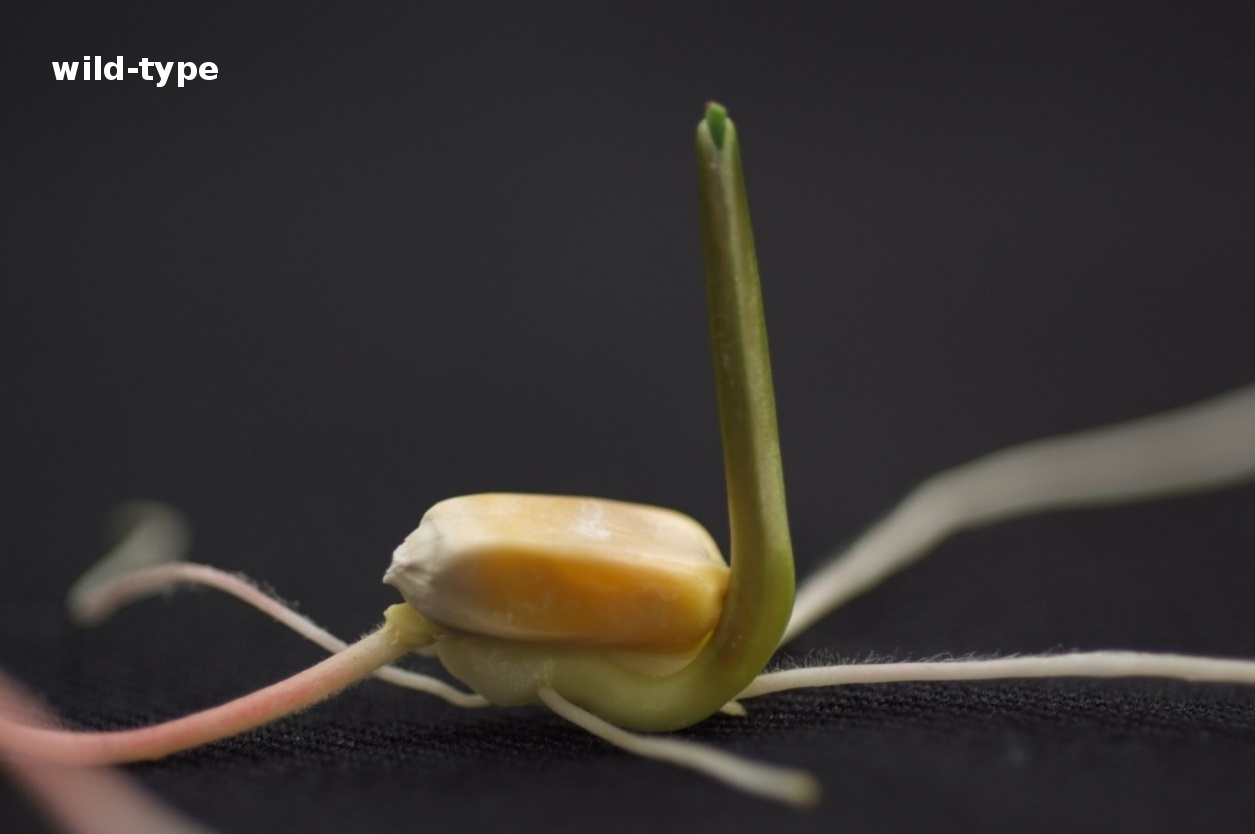
\includegraphics[width=0.5\figwidth]{Tang-seedling-wt}
      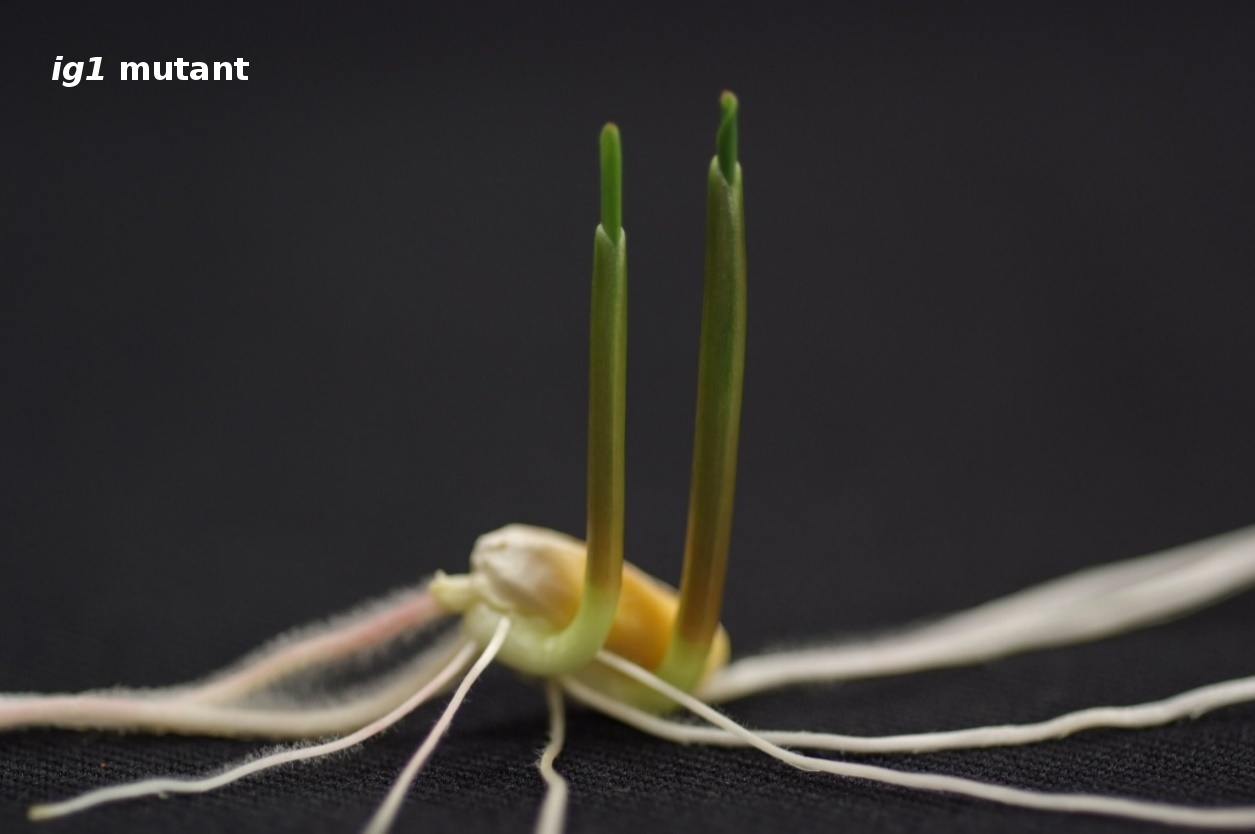
\includegraphics[width=0.5\figwidth]{Tang-seedling-twin}
    \end{minipage}
    \captionof*{figure}{
      Twin seedlings grow from an \textit{ig1} mutant twin-embryo seed.
    }
  \end{center}

  \subsection*{Rate of occurrence}

  The Mo17/B73 hybrid \textit{ig1} mutants exhibit a twinning phenotype at a frequency intermediate between the frequency of
  twinning in individual inbred lines.

  \begin{center}
    \begin{tabular}{|c|c|c|}
      \hline
      \textit{ig1} inbred lines & \# seeds & twins \\
      \hline
      B73 & 1372 & 0.5\% \\
      Mo17/B73 hybrid & 5217 & 4.2\% \\
      Mo17 & 840 & 8.5\% \\
      \hline
    \end{tabular}
  \end{center}

  This suggests a model in which B73 and Mo17 differ for a single modifier with a major
  effect on twinning (the Mo17 allele of this modifier promoting twinning in \textit{ig1} mutants).

  \section*{GBS MAPPING POPULATION}
  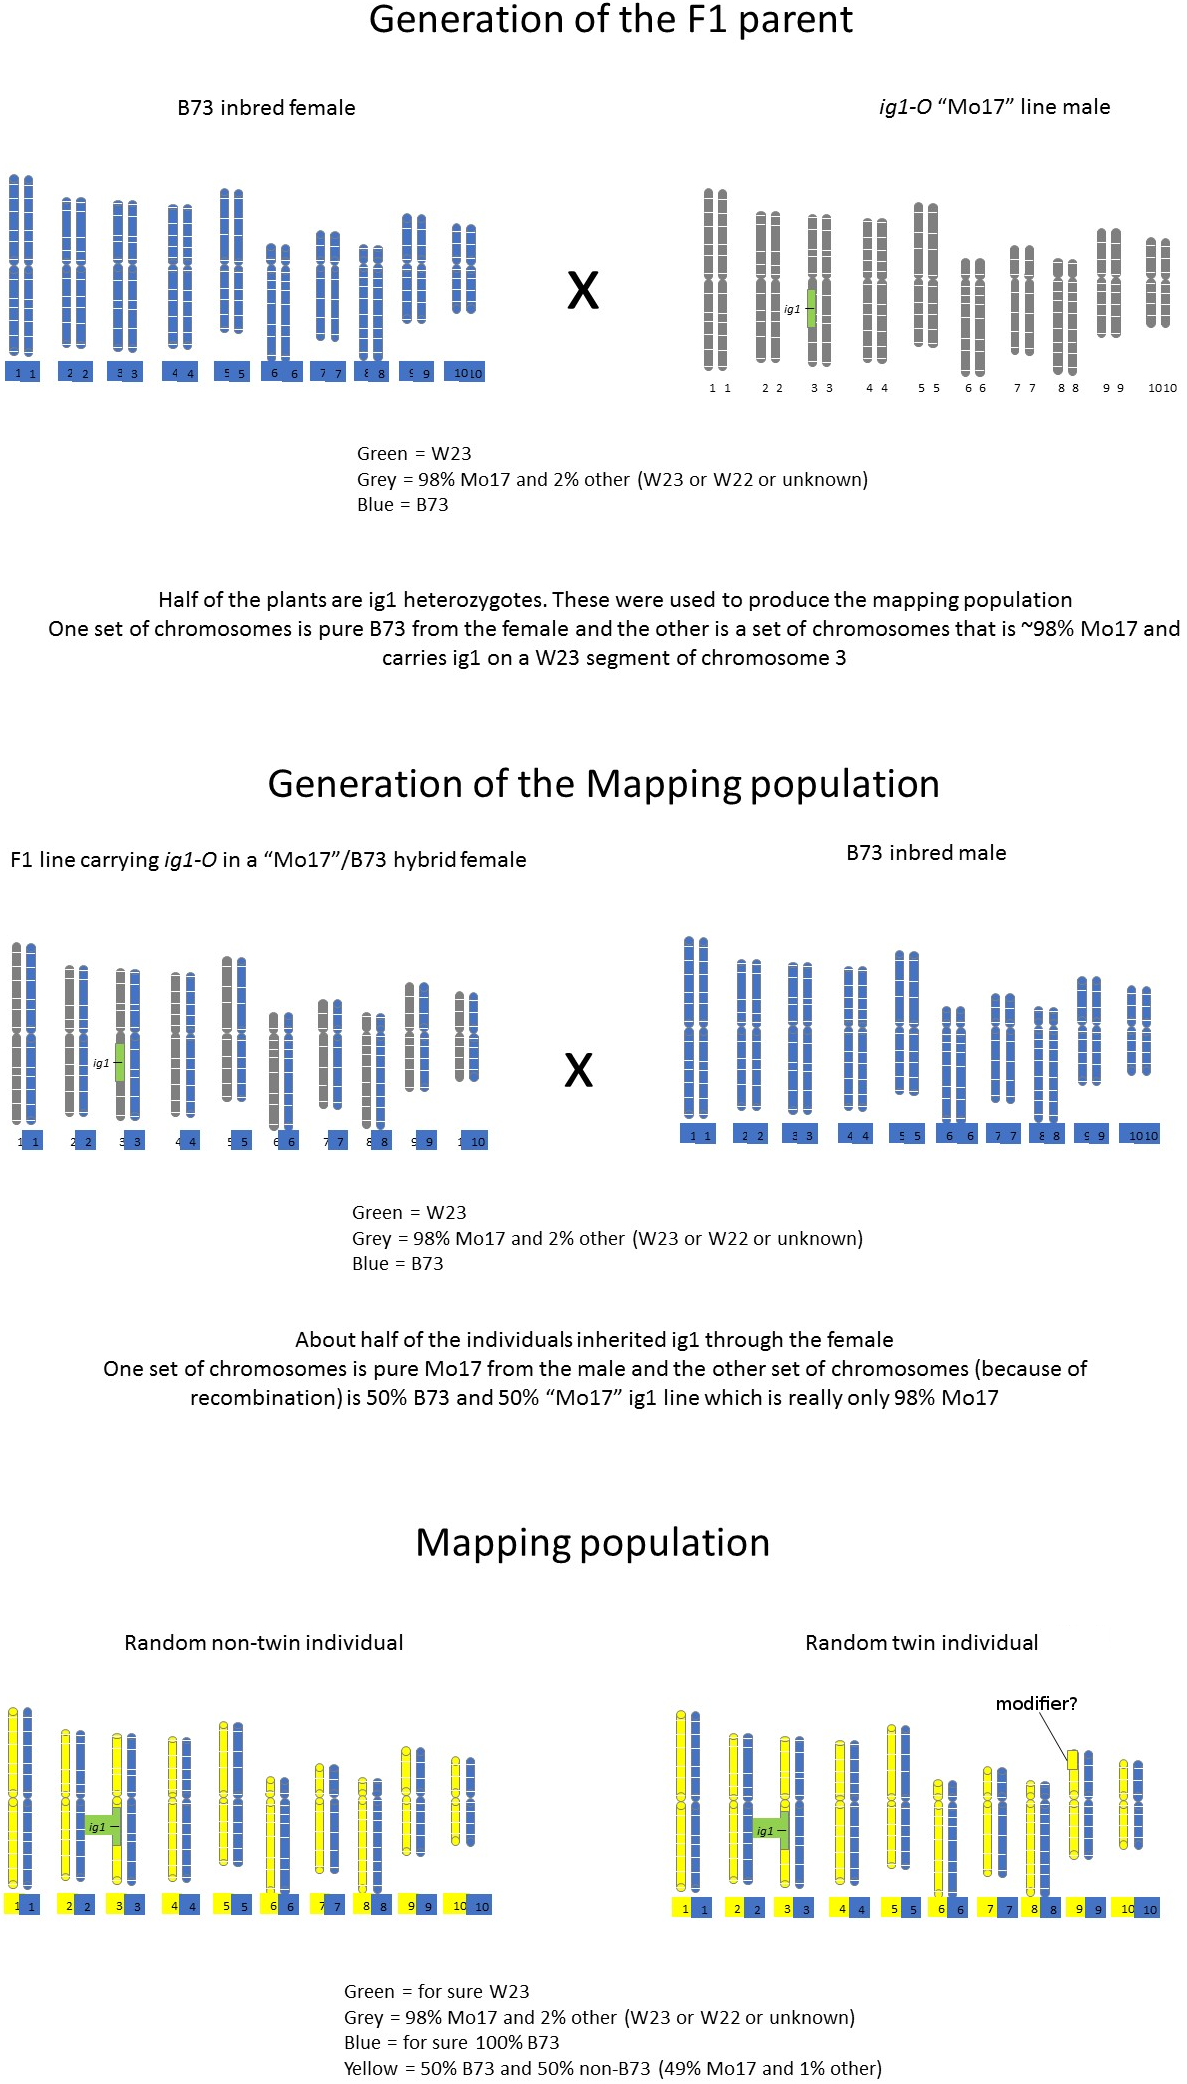
\includegraphics[width=\figwidth]{twin-study-mapping.png}
  
  \section*{GBS RESULTS}

  \subsection*{Mapping and SNP statistics}

  45 sequenced samples had non-twin phenotype, 48 had twin phenotype.
  
  \begin{center}
    \small
    \begin{tabular}{|c|c|c|c|c|}
      \hline
      93 samples & mean & s.d. & max & min \\
      \hline
      mapped reads & 3,633,114 & 676,410 & 5,204,340 & 1,956,272 \\
      \# SNPs & 85,118 & 16,892 & 132,620 & 54,132 \\
      avg. depth & 8.79 & 1.06 & 11.02 & 6.04 \\
      \# > 1x & 2.86\% & 0.24 & 3.61\% & 2.27\% \\
      \# > 4x & 1.62\% & 0.15 & 1.96\% & 1.10\% \\
      Het rate & 0.026\% & 0.005 & 0.039\% & 0.017\% \\
      \hline
    \end{tabular}
  \end{center}

  The GBS sequencing was done by Novogene. The reads were mapped against the B73v4 genome. Positions with at least four reads qualified for SNP calls.

  \subsection*{Example non-segregated and segregated loci}

  Example regions in which roughly half of the samples have heterozygous SNP calls.
  
  \begin{minipage}[t]{0.48\linewidth}
    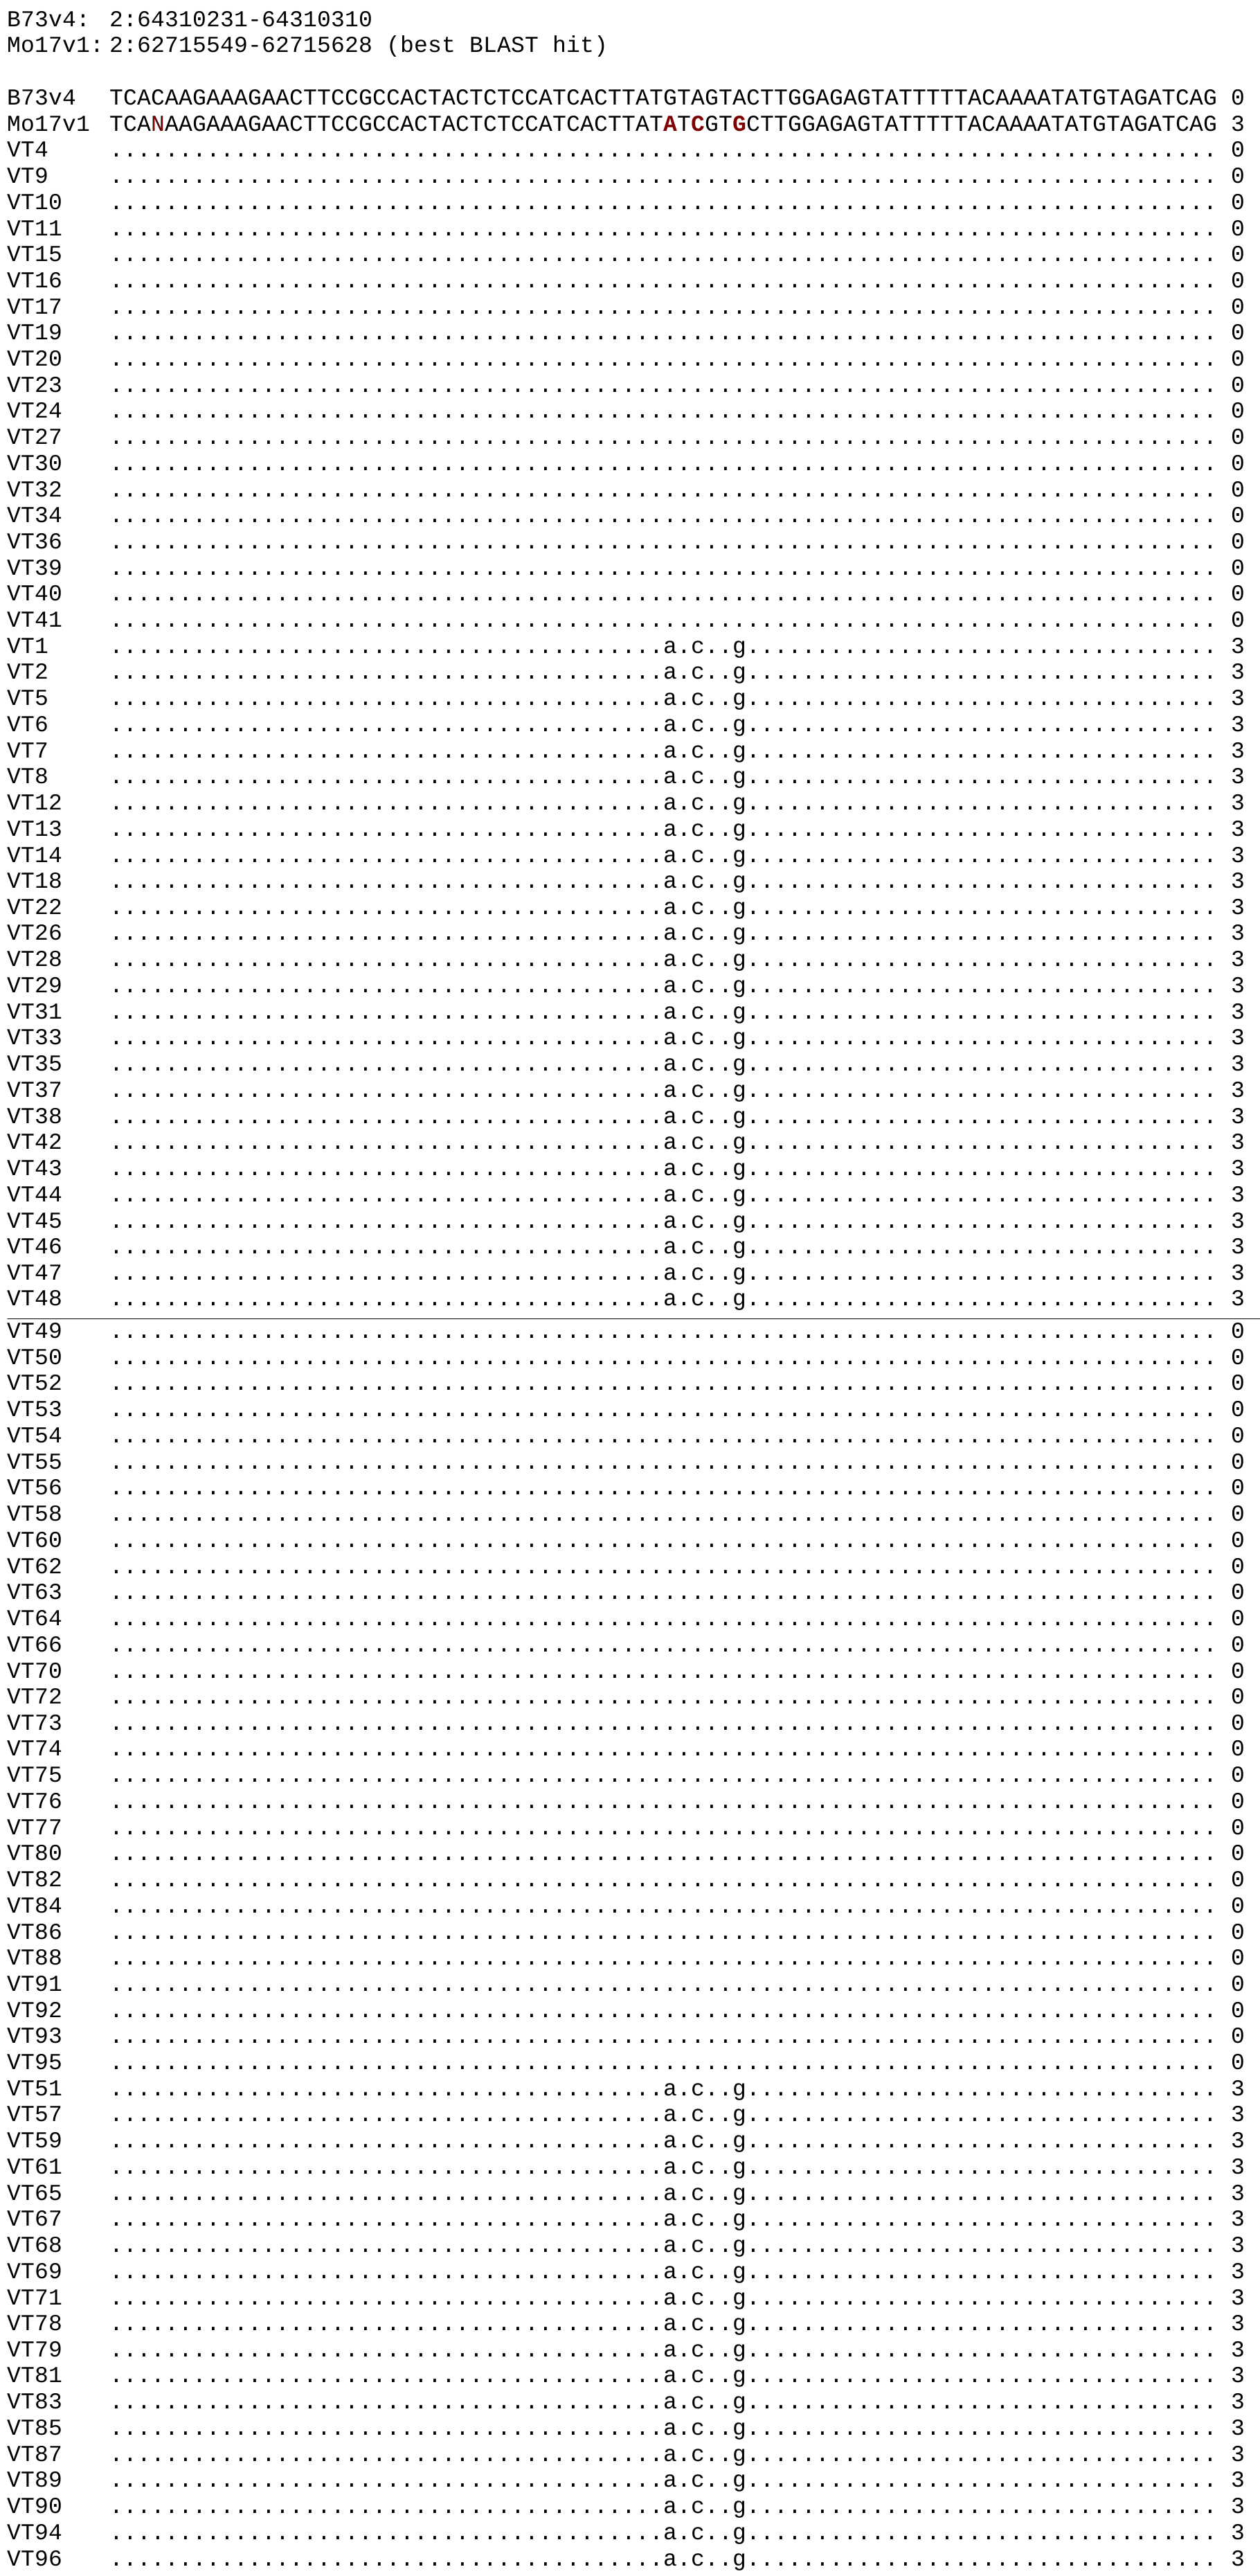
\includegraphics[width=0.48\figwidth]{2.64310231-64310310.png}
    \captionof*{figure}{
      There is no segregation of twins vs. non-twins in this region.
      The three SNPs match the corresponding Mo17v1 best-BLAST-hit region.
    }
  \end{minipage}
  \begin{minipage}[t]{0.04\linewidth}
    \hfill
  \end{minipage}
  \begin{minipage}[t]{0.48\linewidth}
    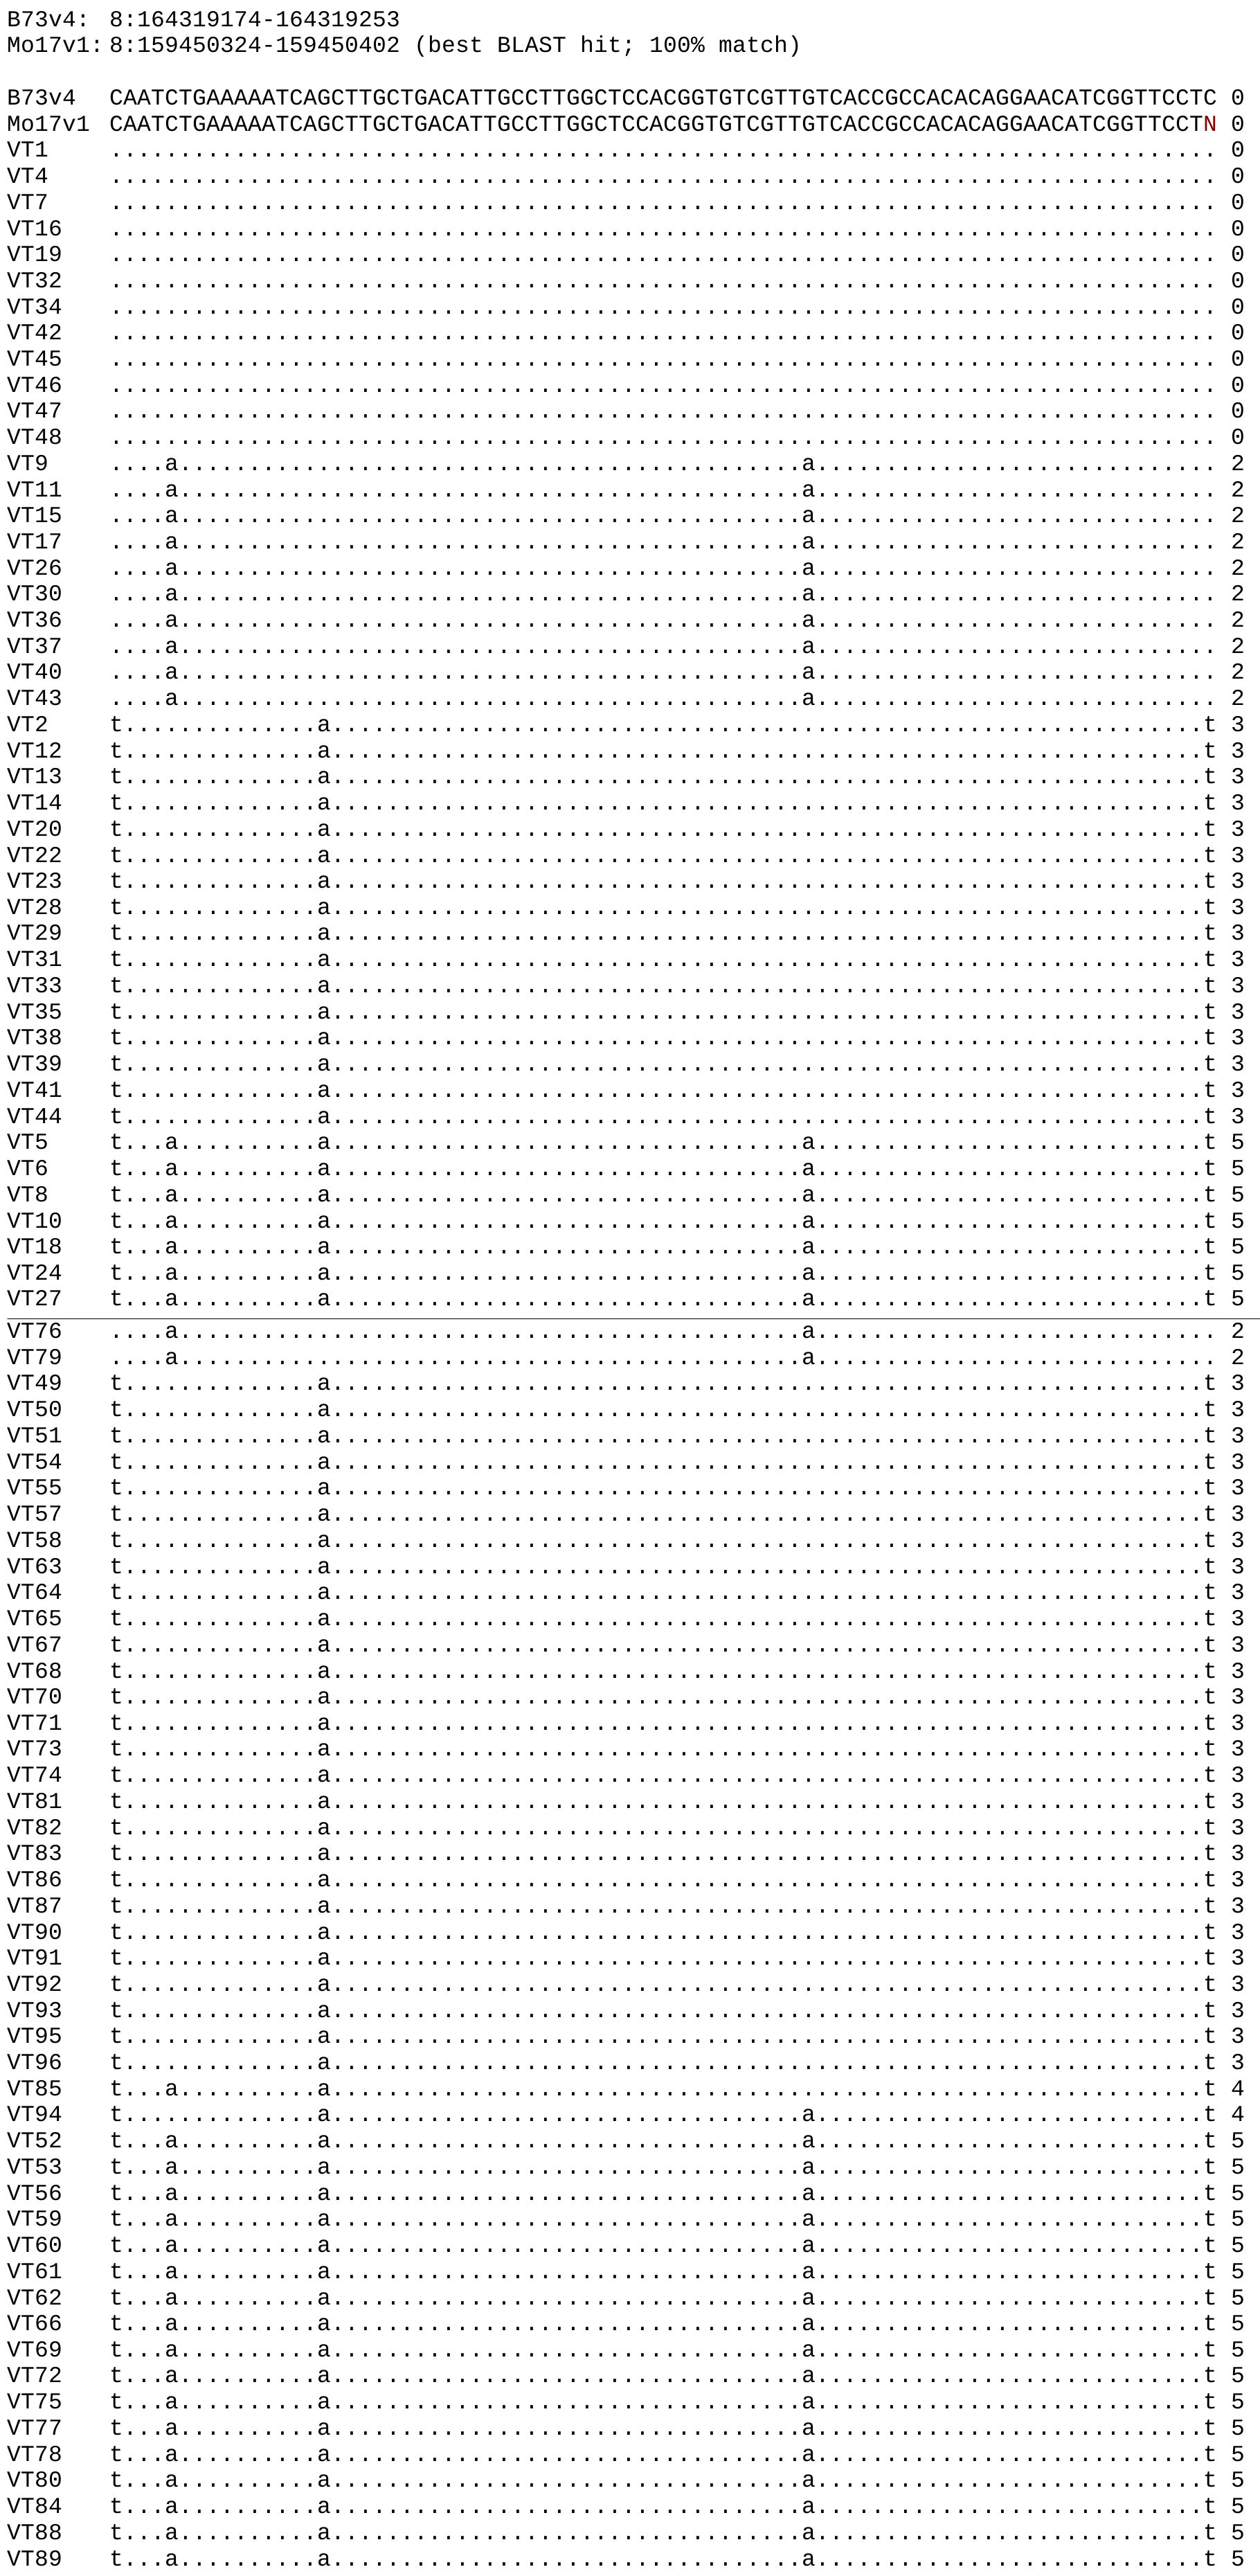
\includegraphics[width=0.48\figwidth]{8.164319174-164319253.png}
    \captionof*{figure}{
      Twin samples segregate significantly from non-twin samples in this region, with more twins carrying three SNPs, which don't match Mo17v1.
    }
  \end{minipage}
    
  \subsection*{Fisher's exact test}

  Each SNP location on the genome provides a classic 2 X 2 contingency table, twin/non-twin vs. het/no call, appropriate for Fisher's Exact Test. Fisher's Exact Test was therefore applied to
  every location, generating a $p$-value at every position. For example:

  \begin{center}
    \begin{tabular}{|r|c|c|c|}
      \hline
      \textbf{2:28422677} & reads & no call & het call \\
      \hline
      non-twin   & 417   & \textbf{27} & 18 \\
      \hline
      twin       & 773   & 7  & \textbf{41} \\
      \hline
      total      & 1190  & 34 & 59 \\
      \hline
    \end{tabular}
    \captionof*{table}{
      Fisher's exact test on calls at this locus gives $p=5.5\times10^{-6}$.
      The number of called samples, 59, and the average reads per called sample, 1190/59=20.2, pass the filter used for the whole-genome Manhattan plot below.
    }
  \end{center}


  \subsection*{Regions of segregation}

  Fisher's exact test was applied to all calls in the GBS study for the null hypothesis that the number of Het calls does not differ between the twin and non-twin groups.
  Loci were plotted if they had at least 4 reads per called sample and had at least 45 Het calls out of 93 samples.
  
  \begin{center}
    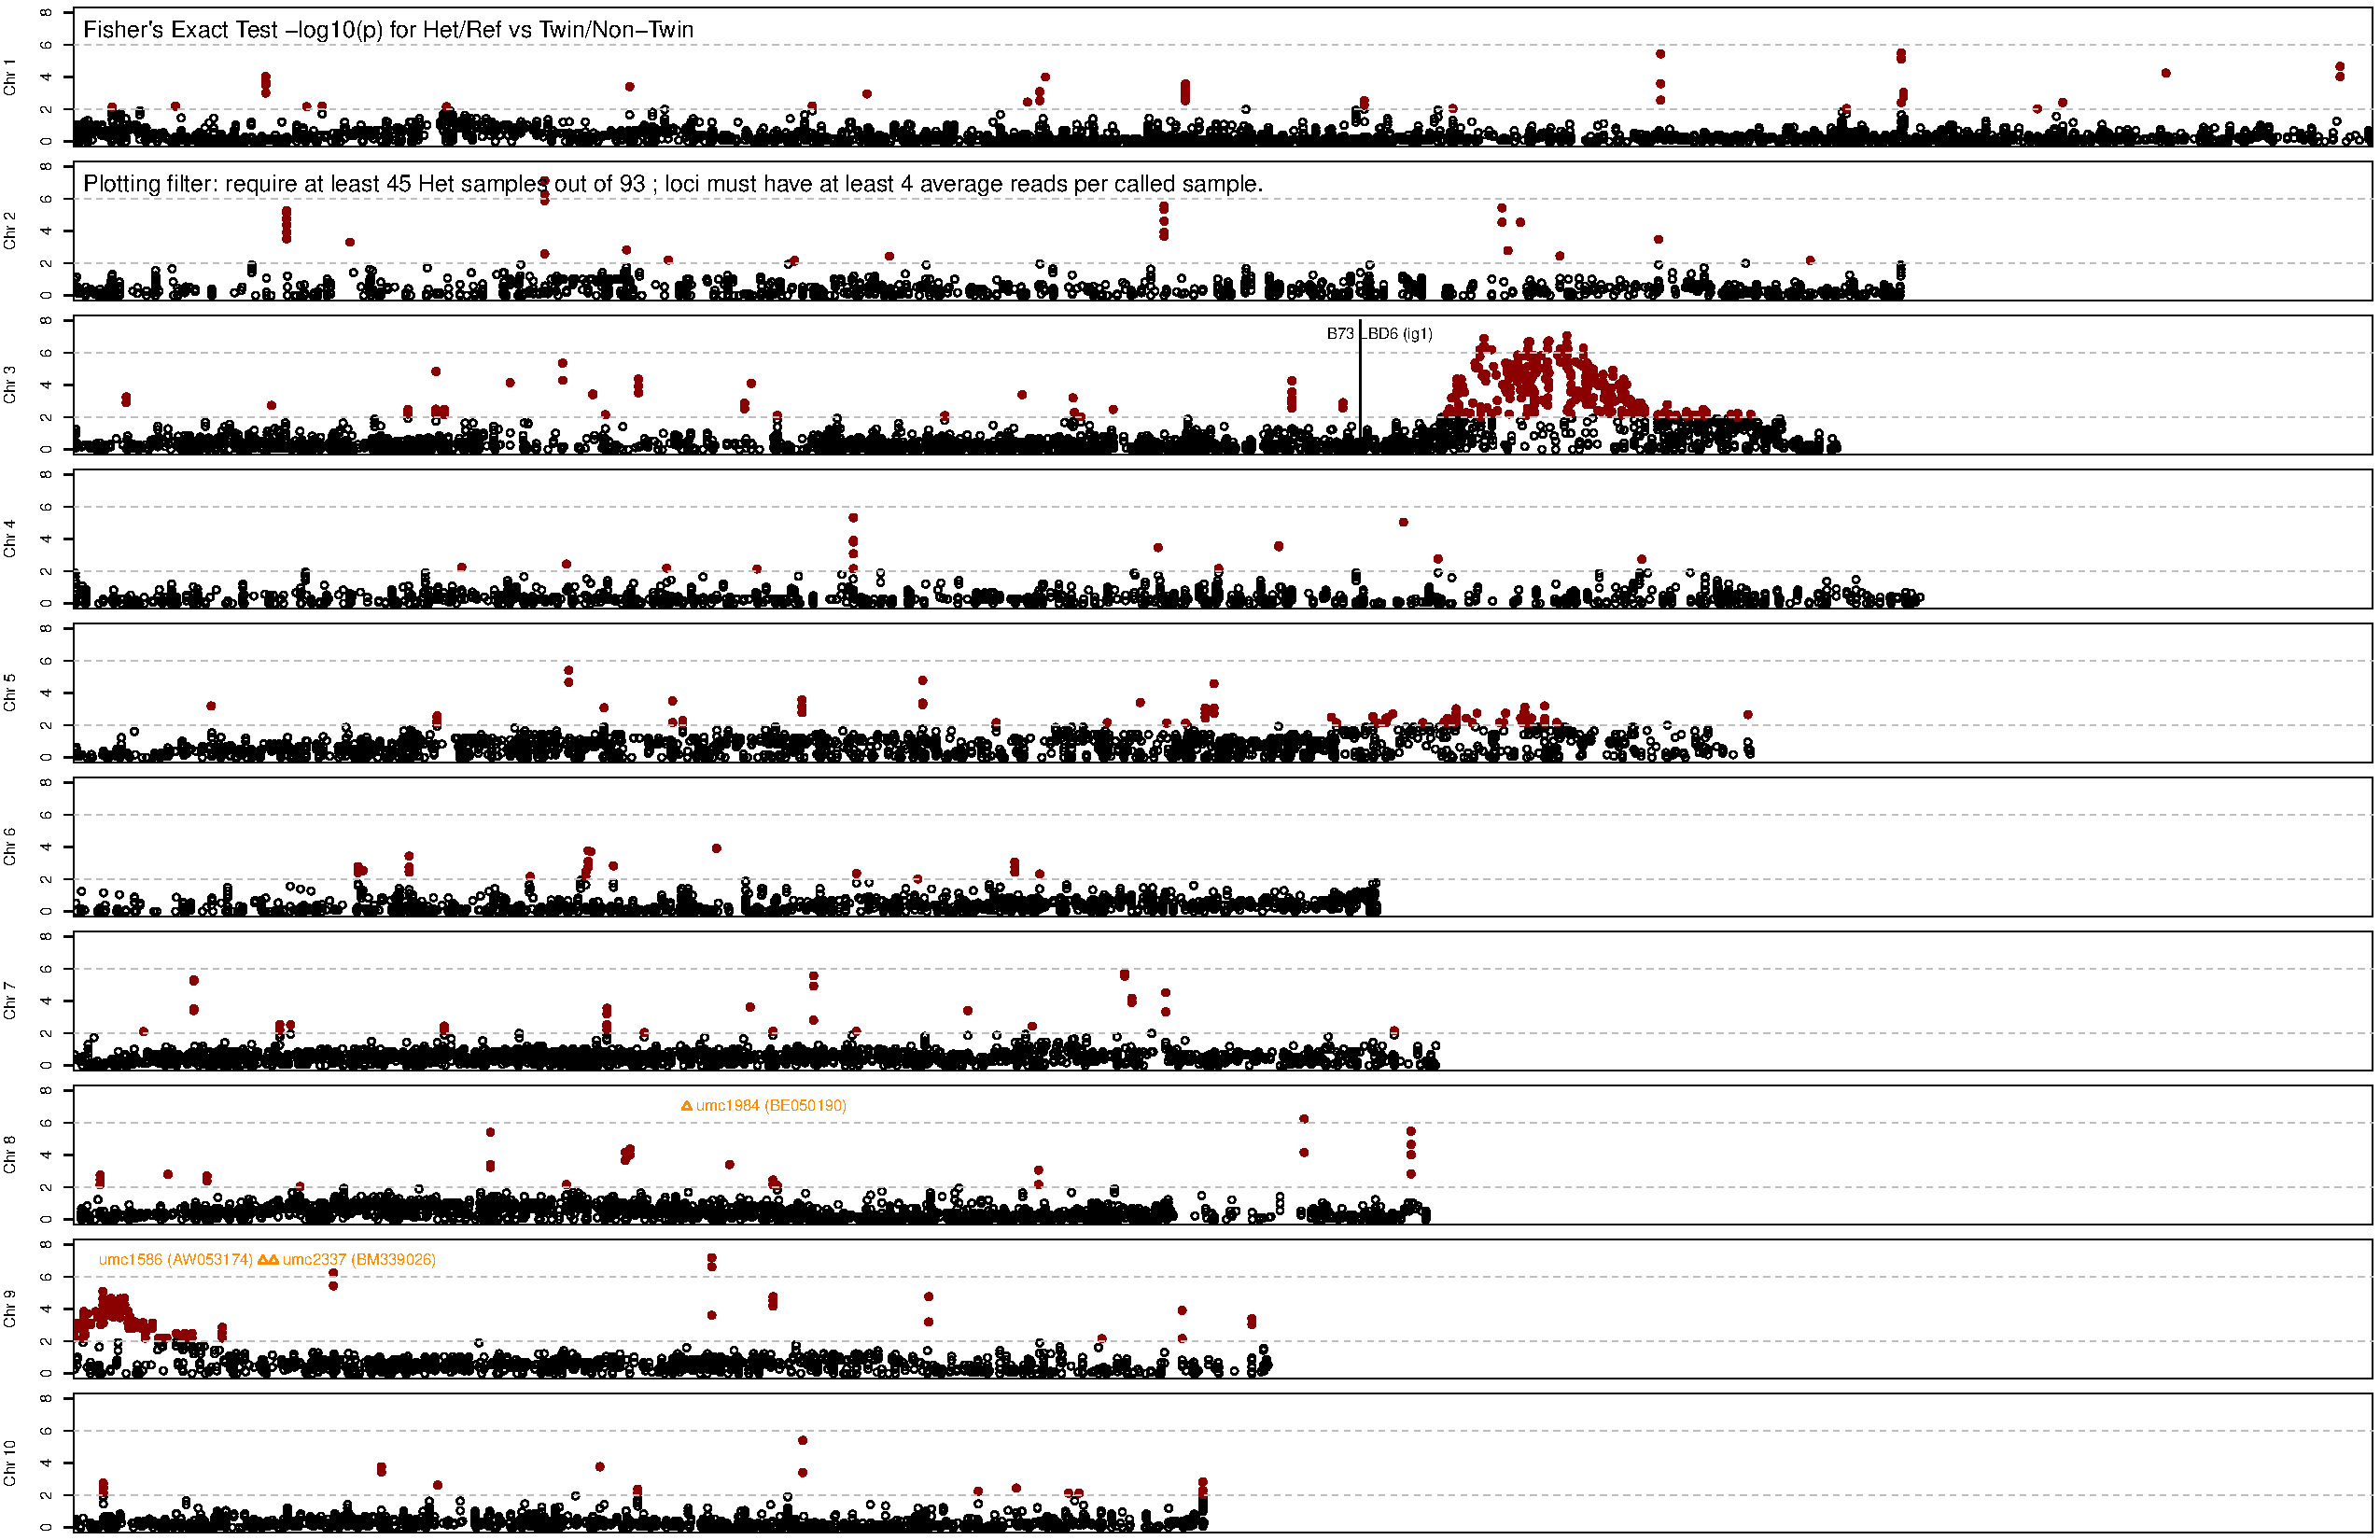
\includegraphics[width=\figwidth]{Fisher-Het-45}
    \captionof*{figure}{
      The position of the LBD6 (\textit{ig1}) gene on Chr3 is indicated, as well as the locations of SSR markers that exhibit segregation between twins and non-twins.
      Red indicates significance at $p<0.01$. Dashed lines are drawn at $p=10^{-2}$ and $10^{-6}$.
    }
  \end{center}


  \section*{SSR MARKERS}

  For comparison to the GBS results, SSR markers on Chr8 and Chr9 were applied to 73 DNA samples of \textit{ig1}
  twins from different plants and progenitor wild-type inbred lines to identify the parental alleles for each locus.
  Of the primers ordered and tested, those for \textbf{umc1984} on Chr8, and \textbf{umc1586} and \textbf{umc2337} on Chr9
  were polymorphic between B73 and Mo17 and showed the clearest bands.
  
  On Chr8, \textbf{umc1984} showed a significantly higher number of heterozygous
  samples than expected ($p<0.05$, chi-squared test), while on Chr9, both \textbf{umc1586} and \textbf{umc2337}
  showed a significantly higher number of heterozygous samples than expected ($p<0.01$, and $p<0.05$, respectively).

  More fine mapping will need to be done to narrow down the modifying regions and to identify candidate genes for
  these enhancers and determine the differences between the B73 and Mo17 alleles.

  \section*{CONCLUSIONS}


  %----------------------------------------------------------------------------------------
  %	REFERENCES
  %----------------------------------------------------------------------------------------

  \nocite{*} % Print all references regardless of whether they were cited in the poster or not
  \bibliographystyle{plain} % Plain referencing style
  \bibliography{hokin-maize2018} % Use hokin-maize2018.bbl - regenerate with bibtex

  %----------------------------------------------------------------------------------------
  %	ACKNOWLEDGEMENTS
  %----------------------------------------------------------------------------------------

  {\small This research was funded by National Science Foundation grant \#XXXXXXX.}
  
  
\end{multicols}
\end{document}
